\documentclass[12pt]{report}
\usepackage[parfill]{parskip}
\usepackage[utf8]{inputenc}
\usepackage{graphicx}
\usepackage{amsthm}
\usepackage{amsmath}
\usepackage{amsfonts}
\usepackage{braket}
\usepackage{xcolor}

\graphicspath{ {figures/} }

\title{
{Title}\\
% {\large A Thesis \\presented to \\ the Faculty of California Polytechnic State University, \\San Luis Obispo}\\
}
\author{Max Varverakis}
\date{\today}

% MATH STUFF
% \renewcommand\qedsymbol{$\blacksquare$}
\newcommand{\ehat}{\hat{e}}
\newcommand{\mat}[3]{{{#1}^#2}_#3}
\newcommand{\sotwo}{\textrm{SO}{(2)}}
\newcommand{\C}{\mathbb{C}}
\newcommand{\R}{\mathbb{R}}
\newcommand{\Z}{\mathbb{Z}}
\newcommand{\D}{\mathbb{D}}
\newcommand{\Q}{\mathbb{Q}}
\newcommand{\iv}[1]{{ #1 }^{-1}}
\newcommand{\aut}[1]{\textrm{Aut}\!\left( #1 \right)}
% \newcommand{\behat}[1]{\bra{\hat{e}[#1]}}
% \newcommand{\kehat}[1]{\ket{\hat{e}[#1]}}

\newtheorem{theorem}{Theorem}[chapter]
\newtheorem{corollary}{Corollary}[theorem]
\newtheorem{lemma}[theorem]{Lemma}

\theoremstyle{definition}
\newtheorem{definition}{Definition}[chapter]
\newtheorem{example}{Example}[chapter]

\begin{document}

\maketitle

\chapter{Representation Theory Background}

\begin{definition}[Representations of a Group]
    If there is a homomorphism from a group $G$ to a group of operators $U(G)$ on a linear vector space $V$, we say that $U(G)$ forms a \textit{representation} of $G$ with dimension $\dim V$.
\end{definition}

The representation is a map
\begin{equation}
    g\in G\xrightarrow{U} U(g)
\end{equation}
in which $U(g)$ is an operator on the vector space $V$. For a set of basis vectors $\{\hat{e_i},i=1,2,\dots,n\}$, we can realize each operator $U(g)$ as an $n\times n$ matrix $D(g)$.
\begin{equation}
    U(g)\ket{e_i} = \sum_{j=1}^n \ket{e_j}{{D(g)}^j}_i = \ket{e_j}{{D(g)}^j}_i,
\end{equation}
where the first index $j$ is the row index and the second index $i$ is the column index. We use the Einstein summation convention, so repeated indices are summed over. Note that the operator multiplication is defined as
\begin{equation}
    U(g_1)U(g_2) = U(g_1g_2),
\end{equation}
which satisfies the group multiplication rules.

\begin{definition}
    If the homomorphism defining the representation is an isomorphism, then the representation is \textit{faithful}. Otherwise, it is \textit{degenerate}.
\end{definition}

\begin{example}
    Let $G$ be the group of continuous rotations in the $xy$-plane about the origin. We can write $G = \{R(\phi),0\leq\phi\leq2\pi\}$ with group operation $R(\phi_1)R(\phi_2) = R(\phi_1+\phi_2)$. Consider the 2-dimensional Euclidean vector space $V_2$. Then we define a representation of $G$ on $V_2$ by the familiar rotation operation
    \begin{align}
        \hat{e}_1' &= U(\phi)\hat{e}_1 = \hat{e}_1\cdot\cos\phi + \hat{e}_2\cdot\sin\phi\\
        \hat{e}_2' &= U(\phi)\hat{e}_2 = -\hat{e}_1\cdot\sin\phi + \hat{e}_2\cdot\cos\phi.
    \end{align}
This gives us the matrix representation
\begin{equation}
    D(\phi) = \begin{pmatrix}
        \cos\phi & -\sin\phi\\
        \sin\phi & \cos\phi
    \end{pmatrix}.
\end{equation}
To further illustrate this representation, if we consider an arbitrary vector $\hat{e_i}x^i=\vec{x}\in V_2$, then we have
\begin{equation}
    \vec{x}' = U(\phi)\vec{x} = \hat{e}_j{x'}^j,
\end{equation}
where ${x'}^j = {{D(\phi)}^j}_i x^i$.
\end{example}

\begin{definition}[Equivalence of Representations]
    For a group $G$, two representations are \textit{equivalent} if they are related by a similarity transformation. Equivalent representations form an equivalence class.
\end{definition}

To determine whether two representations belong to the same equivalence class, we define
\begin{definition}[Characters of a Representation]
    The \textit{character} $\chi(g)$ of an element $g\in G$ in a representation $U(g)$ is defined as $\chi(g) = \text{Tr}~D(g)$.
\end{definition}
Since trace is independent of basis, the character serves as a class label.

Vector space representations of a group have familiar substructures, which are useful in constructing representations of the group.
\begin{definition}[Invariant Subspace]
    Let $U(G)$ be a representation of $G$ on a vector space $V$, and $W$ a subspace of $V$ such that $U(g)\ket{x}\in W$ for all $\vec{x}\in W$ and $g\in G$. Then $W$ is an \textit{invariant subspace} of $V$ with respect to $U(G)$. An invariant subspace is \textit{minimal} or \textit{proper} if it does not contain any non-trivial invariant subspace with respect to $U(G)$.
\end{definition}

The identification of invariant subspaces on vector space representations leads to the following distinction of the representations.
\begin{definition}[Irreducible Representation]
    A representation $U(G)$ on $V$ is \textit{irreducible} if there is no non-trivial invariant subspace in $V$ with respect to $U(G)$. Otherwise, it is \textit{reducible}. If $U(G)$ is reducible and its orthogonal complement to the invariant subspace is also invariant with respect to $U(G)$, then the representation is \textit{fully reducible}.
    
\end{definition}

\begin{example}
    Under the group of 2-dimensional rotations, consider the 1-dimensional subspace spanned by $\ehat_1$. This subspace is not invariant under 2-dimensional rotations, because a rotation of $\ehat_1$ by $\pi/2$ results in the vector $\ehat_2$ that is clearly not in the subspace spanned by $\ehat_1$. A similar argument shows that the subspace spanned by $\ehat_2$ is not invariant under 2-dimensional rotations.

    However, consider the linear combination of basis vectors
    \begin{equation}
        \ehat_\pm = \frac{1}{\sqrt{2}}\left( \mp\ehat_1 + i\ehat_2 \right),
    \end{equation}
    where $i = \sqrt{-1}$. Then a rotation by angle $\phi$, denoted in operator form as $U(\phi)$, acts on $\ehat_\pm$ by
    \begin{align}
        U(\phi)\ket{\ehat_+} &= U(\phi)\frac{1}{\sqrt{2}}(-\ehat_1 + i\ehat_2) \\
        &= \frac{1}{\sqrt{2}}(-U(\phi)\ket{\ehat_1} + iU(\phi)\ket{\ehat_2}) \nonumber \\
        &= \frac{1}{\sqrt{2}}\left( -\ehat_1\cos\phi - \ehat_2\sin\phi -i\ehat_1\sin\phi + i\ehat_2\cos\phi \right) \nonumber \\
        &= \frac{1}{\sqrt{2}}\left( -\ehat_1(\cos\phi+ i\sin\phi) +i\ehat_2(\cos\phi-i\sin\phi) \right) \nonumber \\
        % &= \frac{1}{\sqrt{2}}\big(\ehat_1(-\cos\phi+i\sin\phi) + \ehat_2(i\cos\phi + \sin\phi)\big) \nonumber \\
        % &= \frac{1}{\sqrt{2}}(-\ehat_1 + i\ehat_2)(\cos\phi - i\sin\phi) \nonumber \\
        & \textbf{Not Done} \nonumber \\
        &= \ehat_+ (\cos\phi - i\sin\phi) \nonumber \\
        &= \ehat_+ e^{-i\phi}, \\
        \textrm{and } U(\phi)\ket{\ehat_-} &= \ehat_- e^{i\phi}.
    \end{align}

\end{example}



The irreducible representation matrices satisfy orthonormality and completeness relations.\textbf{ Thm. 3.5}?

\begin{example}[Generator of $\sotwo$]
    Consider the rotations of a 2-dimensional Euclidean vector space about the origin. Let $\ehat_1$ and $\ehat_2$ be orthonormal basis vectors of this space. Using geometry, we can determine how a rotation by some angle $\phi$, written in operator form as $R(\phi)$, acts on the basis vectors:
    \begin{align}
        R(\phi)\ehat_1 &= \ehat_1\cos\phi + \ehat_2\sin\phi \label{eq:rot_1}\\
        R(\phi)\ehat_2 &= -\ehat_1\sin\phi + \ehat_2\cos\phi.\label{eq:rot_2}
    \end{align}
    In matrix form, we can write
    \begin{equation}
        R(\phi) = 
        \begin{pmatrix}
            \cos\phi & -\sin\phi \\
            \sin\phi & \cos\phi
        \end{pmatrix}
    \end{equation}
    which allows us to write Eqn.~\ref{eq:rot_1} and Eqn.~\ref{eq:rot_2} in a condensed form
    \begin{equation}
        R(\phi)\ehat_i = \ehat_j{{R(\phi)}^j}_i,
    \end{equation}
    where we are summing over $j=1,2$.

    Now, let $\vec{x}$ be an arbitrary vector in the plane. Then $\vec{x}$ has components $x^i$ in the basis $\{\ehat_i\}$, where $i=1,2$. Equivalently, we can write $\vec{x}=\ehat_i x^i$. Then under rotations, $\vec{x}$ transforms in accordance to the basis vectors
    \begin{align}
        R(\phi)\vec{x} &= R(\phi)\ehat_i x^i \label{eq:rot_vec} \\
        &= \ehat_j{{R(\phi)}^j}_i x^i \nonumber \\
        &= \left( \ehat_1\mat{R(\phi)}{1}{i} + \ehat_2\mat{R(\phi)}{2}{i} \right)x^i \nonumber \\
        &= \left( \ehat_1\cos\phi + \ehat_2\sin\phi \right) x^1 + \left( \ehat_1(-\sin\phi) + \ehat_2\cos\phi \right) x^2 \nonumber \\
        &= \left( x^1\cos\phi - x^2\sin\phi \right)\ehat_1 + \left( x^1\sin\phi + x^2\cos\phi \right)\ehat_2.  \nonumber
    \end{align}

    Observe that $R(\phi)R^\top(\phi) = E$ where $E$ is the identity matrix. This is precisely what defines \textit{orthogonal matrices}. For 2-dimensional vectors in the plane, it is clear that these rotations do not change the length of said vectors. This can be verified by using Eqn.~\ref{eq:rot_vec}:
    \begin{align}
        |R(\phi)\vec{x}|^2 &= |\ehat_j\mat{R(\phi)}{j}{i} x^i|^2 \\
        &= \left|\left( x^1\cos\phi - x^2\sin\phi \right)\ehat_1 + \left( x^1\sin\phi + x^2\cos\phi \right)\ehat_2\right|^2 \nonumber \\
        &= {\left( x^1\cos\phi - x^2\sin\phi \right)}^2 + {\left( x^1\sin\phi + x^2\cos\phi \right)}^2 \nonumber \\
        &= \left( \cos^2\phi + \sin^2\phi \right)x^1 x_1 + \left( \sin^2\phi + \cos^2\phi \right)x^2 x_2 \nonumber \\
        &= x^1 x_1 + x^2 x_2 = |\vec{x}|^2. \nonumber
    \end{align}

    Similarly, notice that for any continuous rotation by angle $\phi$, $\det R(\phi) = \cos^2\phi+\sin^2\phi = 1$. In general, orthogonal matrices have determinant equal to $\pm1$. However, the result of the above determinant of $R(\phi)$ implies that all continuous rotations in the 2-dimensional plane have determinant equal to $+1$. These are the \textit{special orthogonal matrices of rank 2}. This family of matrices is denoted $\sotwo$. Furthermore, there is a one-to-one correspondence with $\sotwo$ matrices and rotations in a plane.

    We define the group of continuous rotations in a plane by letting $R(0) = E$ be the identity element corresponding to no rotation (i.e., a rotation by angle $\phi=0$), and defining the inverse of a rotation as $R^{-1}(\phi) = R(-\phi) = R(2\pi-\phi)$. This group can be called the $\sotwo$ group. Lastly, we define group multiplication as $R(\phi_1)R(\phi_2) = R(\phi_1+\phi_2)$ and note that $R(\phi) = R(\phi\pm2\pi)$, which can be verified geometrically. Thus, group elements of $\sotwo$ can be labelled by the angle of rotation $\phi\in[0,2\pi)$.

    Now we can find a generator of $sotwo$ by considering an infinitesimal rotation, labelled by some infinitesimal angle $d\phi$. Then this is equivalent to the identity plus some small rotation, which we can write as
    \begin{equation}
        R(\textrm{d}\phi) = E - i \textrm{d}\phi J
    \end{equation}
    where the scalar quantity $-i$ is introduced for later convenience and $J$ is some quantity independent of the rotation angle. If we consider the rotation $R(\phi + \textrm{d}\phi)$, then there are two equivalent ways to interpret this rotation
    \begin{align}
        R(\phi + \textrm{d}\phi) &= R(\phi)R(\textrm{d}\phi) = R(\phi)(E - i \textrm{d}\phi J) = R(\phi) - i \textrm{d}\phi R(\phi)J \\
        R(\phi + \textrm{d}\phi) &= R(\phi) + \textrm{d}R(\phi) = R(\phi) + \textrm{d}\phi\frac{\textrm{d}R(\phi)}{\textrm{d}\phi}
    \end{align}
    where the second equation can be thought of as a Taylor expansion of $R(\phi + \textrm{d}\phi)$ about $\phi$. Equating the two expressions for $R(\phi + \textrm{d}\phi)$ yields
    \begin{equation}
        \textrm{d}R(\phi) = -i\textrm{d}\phi R(\phi)J.
    \end{equation}
    Solving this differential equation (with boundary condition $R(0)=E$) provides us with an equation for any group element involving $J$:
    \begin{equation}
        R(\phi) = e^{-i\phi J},
    \end{equation}
    where $J$ is called the \textit{generator} of the group.
\end{example}

\chapter{Topological Definitions}
The braid group is formally defined in terms of topology. In order to understand the braid group, we must first understand the underlying topological properties that are used to define the braid group. Similar to an isomorphism in algebra, we can define a notion of equivalence in topology.

\begin{definition}
    Consider $X$ and $Y$ to be two topological spaces. A \textit{homotopy} between two continuous functions $f,g:X\to Y$ is a continuous function $H:X\times[0,1]\to Y$ such that $H(x,0)=f(x)$ and $H(x,1)=g(x)$ for all $x\in X$. If such a homotopy exists, we say that $f$ and $g$ are \textit{homotopic}.
\end{definition}
The homotopy $H$ can be thought of as a continuous deformation of $f$ into $g$. The interval $\left[ 0,1 \right]$ represents the ``time'' parameter of the deformation. At time equal to 0, the function $H$ is equal to $f$, and at time equal to 1, the function $H$ is equal to $g$. If two functions are homotopic, then they belong to the same homotopy class, which is an equivalence class of functions under the relation of homotopy.

\begin{definition}
    A \textit{loop} on a topological space $X$ is a continuous function $\ell:[0,1]\to X$ such that $\ell(0) = \ell(1)$. In other words, the path of $\ell$ starts and ends at the same point in $X$. Often, this point is called the \textit{base point} of the loop.
\end{definition}

\begin{definition}
    A \textit{homotopy class of loops} on a topological space $X$ is an equivalence class of loops under the relation of homotopy. More plainly, a homotopy of loops is a continuous transformation of one loop into another. If two loops $\ell_1,\ell_2:[0,1]\to X$ with base point $\xi\in X$ are homotopic, then there exists a continuous map $H:[0,1]\times [0,1]\to X$ such that:
    \begin{enumerate}
        \item $H(0,t) = \xi = H(1,t)$ for all $t\in [0,1]$, and
        \item $H(s,0) = \ell_1(s)$ and $H(s,1) = \ell_2(s)$ for all $s\in [0,1]$.
    \end{enumerate}
    Property 1 ensures that the starting/ending point of the loop remains fixed throughout the deformation from $\ell_1$ to $\ell_2$, and property 2 follows from the definition of a homotopy.
\end{definition}

\begin{definition}
    The \textit{fundamental group} of a topological space $X$ with base point $\xi$ is defined as the collection of loops on $X$ with base point $\xi$ modulo homotopy. In other words, the fundamental group is the collection of equivalence classes of loops under homotopy. This is written as
    \begin{align*}
        \pi(X,\xi):=\left\{ \textrm{loops }\ell \textrm{ on }X \textrm{ with base point }\xi \right\}/\textrm{homotopy}.
    \end{align*}
    Often times, the base point of a loop is arbitrary, so we can write $\pi(X)$ instead of $\pi(X,\xi)$ to denote the fundamental group of $X$.
\end{definition}

The group structure of the fundamental group is defined as operations on the loops themselves. Consider two loops $\ell_1,\ell_2:[0,1]\to X$ with base point $\xi$. Then the product $\ell_1\cdot\ell_2$ is defined in terms of \textit{concatenation} of the two loops. Specifically, this defines a new loop $(\ell_1\cdot\ell_2)(t)=\mathcal{L}(t):[0,1]\to X$ where $\mathcal{L}(t) = \ell_1(2t)$ on $\left[ 0,\frac{1}{2} \right]$ and $\mathcal{L}(t) = \ell_2(2t-1)$ on $\left[ \frac{1}{2},1 \right]$. Loop concatenation can be thought of as stitching the loops together at the shared base point. As $t$ ranges from 0 to 1, we can think of the first half of the deformation as traversing the first loop at twice the original speed, and then traveling along the second loop at twice the original speed in the second half of the deformation. 

In the above description, recall that each loop $\ell$ is actually an equivalence class $\left[ \ell \right]$ under the relation of homotopy. So the concatenation of two loops $\ell_1$ and $\ell_2$ is actually the concatenation of any two loops belonging to the equivalence classes $\left[ \ell_1 \right]$ and $\left[ \ell_2 \right]$, which becomes the equivalence class $\left[ \ell_1\cdot\ell_2 \right]$.

In the fundamental group, the inverse of an element is the identical topological path traversed in the opposite direction. Hence, if $\gamma:[0,1]\to X$ is a loop on $X$, then $\iv{\gamma}(t) := \gamma(1-t)$.

% \begin{example}
%     Consider a \textbf{3-dimensional(?)} torus $T^3$. The fundamental group of the torus is $\pi(T^3)$. There are two types of loops on the torus: those that pass through the hole of the torus, and those that do not.
% \end{example}

Just as how homotopy describes a continuous transformation from one continuous path on a topological space to another, we can define topological equivalence on a larger scale.
\begin{definition}
    A continuous, bijective function $f:X\to Y$ between two topological spaces $X$ and $Y$ such that the inverse $\iv{f}:Y\to X$ is also continuous and bijective is called a \textit{homeomorphism}. If there exists such a homeomorphism, then we say $X$ is \textit{homeomorphic} to $Y$. Moreover, an \textit{embedding} of topological spaces is a continuous function that is a homeomorphism when restricted to its image. If we have a continuous family of homeomorphisms $f_t:X\to Y$ for $t\in[0,1]$, then we say that $X$ and $Y$ are \textit{isotopic}. The isotopy of $X$ and $Y$ can be written as a function $H:X\times[0,1]\to Y$ such that
    \begin{enumerate}
        \item $H(x,0)=x$ for all $x\in X$, 
        \item $H(x,1)=f(x)$ for all $x\in X$, and
        \item $H(-,t)$ is an embedding of $X$ onto $Y$ for all $t\in[0,1]$.
    \end{enumerate}
\end{definition}
Evidently, isotopy defines a stronger and more broad notion of topological equivalence, which will be important in defining representations later on.

\chapter{The Braid Group}
\begin{definition}
    The \textit{configuration space} of $n$ ordered distinct points in the complex plane $\C$ is defined as $M_n = \left\{ \left( z_1,\dots,z_n \right)\in\C ; z_i\neq z_j,\forall i\neq j \right\}$. Alternatively, consider $\mathcal{D}$ to be the collection of all hyperplanes $H_{i,j}=\left\{ z_i=z_j \right\}\in\C^n$ for $1\leq i < j \leq n$. Then we can define $M_n = \C^n \setminus \mathcal{D}$.
\end{definition}

Note that $\left( z_1,z_2,z_3,\dots,z_n \right)$ and $\left( z_2,z_1,z_3,\dots,z_n \right)$ are different points in the configuration space $M_n$. Before studying the various interpretations of the braid group, we first define the braid group itself.

\begin{definition}
    The \textit{pure braid group} on $n$ strands, denoted $PB_n$, is the fundamental group of $M_n$. One can write $PB_n = \pi_1(M_n)$.
\end{definition}

\section{Visualization of pure braids}

We can think of a pure braid as a loop in $M_n$:
\begin{align*}
    \beta : \left[ 0,1 \right] &\to M_n \\
    t &\mapsto \beta(t) = \left( \beta_1(t),\beta_2(t),\dots,\beta_n(t) \right),
\end{align*}
with some base point. Conventionally, we define the base point as the $n$-tuple of integers $(1,2,3,\dots,n)\in \C^n$. Then a pure braid can be though of the motion of these points in the complex plane as $t$ ranges from 0 to 1 in which $\beta_i(t)$ is defined and $\beta_i(t)\neq \beta_j(t)$ for every $t\in[0,1]$ and $i\neq j\in\left\{ 1,2,\dots,n \right\}$. Because each $\beta_i$ is a loop, it must start and end at the point $i$ (e.g., $\beta_i(0)=\beta_i(1)=i$). Recall that the loops are actually equivalence classes of loops under homotopy. As a result, we can continuously deform the motion of the $n$ points while maintaining the same pure braid (up to equivalence) so long as we preserve the pairwise distinction of the points for all time $t\in[0,1]$.

A common visualization of pure braids is to plot the motion of the points in 3-dimensional space. For each $t\in [0,1]$, we draw the points $\left( \beta_i(t),t \right)$ in $\C\times[0,1]$ for every $i\in\left\{ 1,\dots,n \right\}$. The space $\C\times[0,1]$ can be thought of as a spacetime diagram, where the motion of the points is plotted in the complex plane at each time $t$, with the time being the vertical axis. The convention is to have $\C\times\left\{ 0 \right\}$ placed above $\C\times\left\{ 1 \right\}$, so that the motion of the points is plotted from top to bottom.

For every $i\in\left\{ 1,\dots,n \right\}$, the motion of a single point starting at $(i,0)$ and ending at $(i,1)$ is known as the $i$-th \textit{strand} of the pure braid. This can also be described by the $i$-th projection of the $n$-tuple $\beta(t)$. Thus, two braids are equivalent under homotopy if, for every moment of a continuous deformation of the $n$ strands in $\C\times [0,1]$, the (fixed) endpoints $((1,0),(2,0),\dots,(n,0))$ and $((1,1),(2,1),\dots,(n,1))$ are connected by strands that are pairwise disjoint where each strand intersects the plane $\C\times\left\{ t \right\}$ exactly once for every $t\in[0,1]$.

As pure braids are members of the pure braid group, multiplication is a well-defined operation. In the context of $M_n$, multiplication of pure braids involves the concatenation of loops. Visually, this is the process of stacking braids on top of each other, and then rescaling the time dimension so that $t$ ranges from 0 to 1.

\section{General braids}
In the previous section, we defined pure braids in which the endpoints of each strand are identical at the beginning and end of the motion. This notion generalizes to define (non-pure) braids. First, we define a more general configuration space than $M_n$. The symmetric group $S_n$ permutes the $n$ distinct points in $\C$. Then the \textit{configuration space of n unordered points in $\C$} is the quotient space $N_n = M_n/S_n$.

\begin{definition}
    The braid group on $n$ strands is the fundamental group of $N_n$, denoted $B_n = \pi_1(N_n)$.
\end{definition}

The visualization of a braid is the same as in the case of pure braids, only now the endpoints of each strand do not necessarily match the starting points. For example, the $i$-th strand may start at the point $(i,0)$ but end at the point $(j,1)$ for $i,j\in\left\{ 1,\dots,n \right\}$. The equivalence of strands is still defined as before under the homotopy of loops. Loop concatenation defines the multiplication of braids, as before.

\section{Standard generators of the braid group}\label{sec:std_gens}
Originally proposed by Artin~\cite{Artin1947}, each braid can be decomposed into a product of \textit{standard generators} of the braid group. When visualizing braids in $\R\times[0,1]$, a crossing of two strands is clearly indicated by one going over the other. Suppose each crossing occurs at a different time $t\in[0,1]$. Then by rescaling the time component of an arbitrary braid, we can deconstruct it into a stack of simple braids with only one crossing between neighboring strands per braid. Each single crossing of strands can be obtained by performing a transposition between neighboring endpoints of the strands.

For instance, swapping the endpoints of the $i$-th and $(i+1)$-th strands can be written as applying $\sigma_i$ to the identity braid (i.e., the braid that starts without any crossings of strands). It must be noted that there are two distinct ways to swap the endpoints of two strands. From a bottom-up perspective looking at just $\C\times\left\{ 1 \right\}$, $\sigma_i$ swaps $(i,1)$ and $(i+1,1)$ in a counterclockwise rotation. The reverse of this operation (i.e., twisting the endpoints around in the clockwise direction) is denoted $\sigma_i^{-1}$. The standard generators of the braid group $B_n$ are defined as the set $\left\{ \sigma_1,\sigma_2,\dots,\sigma_{n-1} \right\}$. An arbitrary braid can be constructed by concatenating (or stacking) the simple braids made from the standard generators before rescaling the time coordinate to $[0,1]$.

\section{Automorphisms of the free group}

Consider the $n$-times punctured disk $\D_n$. The fundamental group of $\D_n$ involves loops that start and end at the same (fixed) base point in $\partial\D_n$. Up to homotopy, a clockwise loop that only encompasses the $i$-th hole in $\D_n$ is analogous to the $i$-th generator of the free group $F_n$ of rank $n$. In fact, we have $\pi_1\left( \D_n \right) = F_n$. This equality allows us to define a representation of the braid group on $n$ strands as automorphisms of $F_n$.

Each braid $\beta\in B_n$ is realized as an automorphism of $\pi_1(\D_n) = F_n$ (up to isotopy) in which each loop $\gamma\in\pi_1(\D_n)$ is sent to another loop $\beta(\gamma)$. In other words, we have a representation of the braid group defined by
\begin{align}
    \rho: B_n &\to \aut{F_n} \\
    \beta &\mapsto \rho_\beta.
\end{align}
The action of $\beta$ on a loop $\gamma$ is defined by the rearrangements of the $n$ holes in $\D_n$, similar to the action of the standard generators of $B_n$ on the base points in $\C\times\left\{ 1 \right\}$. In terms of the standard generators of $B_n$, each $\sigma_i$ corresponds to switching the places of hole $i$ and hole $i+1$ by means of a counterclockwise rotation, as seen in Figure~\ref{fig:sigma_on_Dn}. This is identical to viewing the action of $\sigma_i$ on the base points in $\C\times\left\{ 1 \right\}$ from the bottom-up, as described in Section~\ref{sec:std_gens}. As before, the inverse action $\iv{\sigma_i}$ is a clockwise rotation of the two adjacent holes $i$ and $i+1$ in $\D_n$. These actions respect the group operation of loop concatenation.

\begin{figure}[htbp]
    \centering
    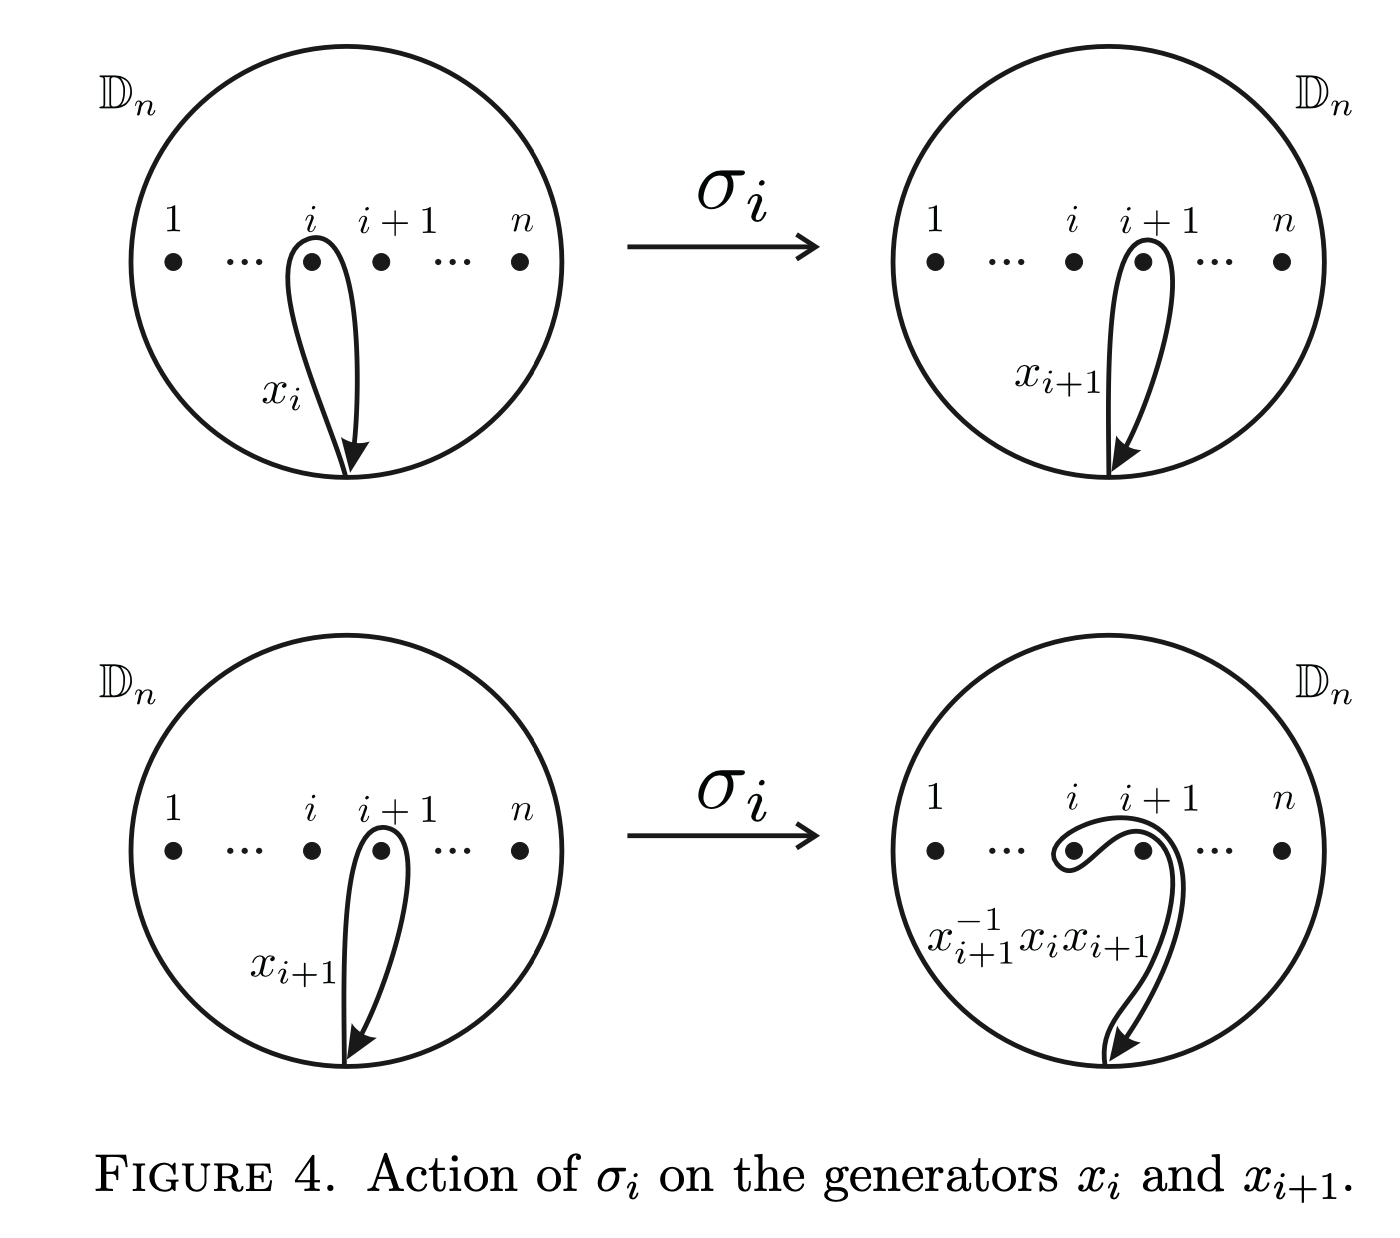
\includegraphics[width = .5\textwidth]{Gonzalez_Fig4_sigma_on_Dn.png}
    \caption{\colorbox{red}{Replace}}\label{fig:sigma_on_Dn}
\end{figure}

The automorphism $\rho_\beta$ is most simply defined in terms of the action of the standard generators of $B_n$ on the generators $x_1,\dots,x_n$ of $F_n$ (visualized as loops in $\D_n$). For each $i\in\left\{ 1,\dots,n-1 \right\}$, it follows that
\begin{align}
    &\rho_{\sigma_i}(x_i) = x_{i+1}, \\
    &\rho_{\sigma_i}(x_{i+1}) = \iv{x_{i+1}}x_i x_{i+1}, \\
    &\rho_{\sigma_i}(x_j) = x_j, \textrm{ for } j\neq i,i+1.
\end{align}
These relations can be verified graphically as in Figure~\ref{fig:sigma_on_x_i}.
\begin{figure}[htbp]
    \centering
    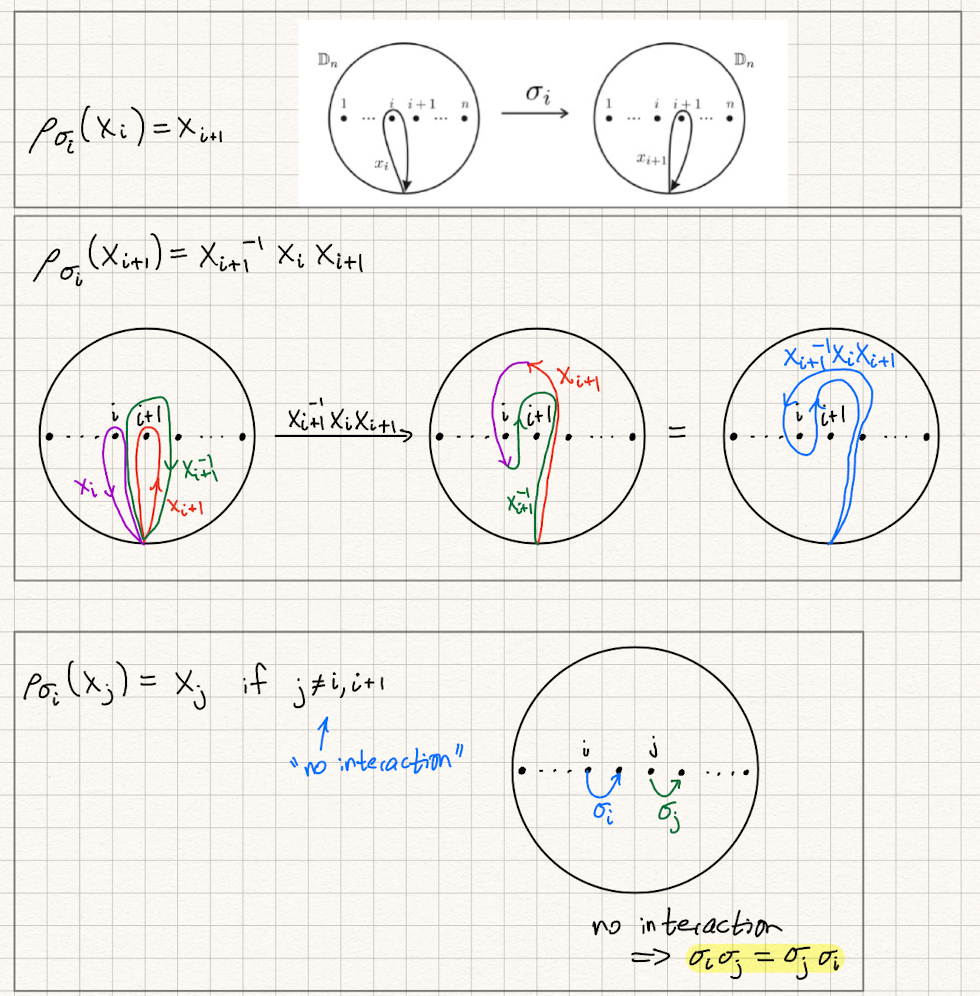
\includegraphics[width = .5\textwidth]{sketch_sigma_on_x_i.png}
    \caption{\colorbox{red}{CAPTION}}\label{fig:sigma_on_x_i}
\end{figure}
For any $\sigma_i$, $\rho_{\iv{\sigma_i}}$ is clearly defined. It follows that for any braid $\beta\in B_n$, we can decompose $\rho_\beta$ the composition of the automorphisms of the standard generators $\sigma_1,\dots,\sigma_{n-1}$ and their inverses that make up $\beta$. 

Notice that for any $\sigma_i$, $\rho_{\sigma_i}(x_1\cdots x_n) = x_1\cdots x_n$. This is because the loop $x_1\cdots x_n$ in $\D_n$, encompassing all holes, is parallel to the boundary $\partial\D_n$. Thus, the action of $\sigma_i$ on $x_1\cdots x_n$ is trivial does not affect the structure of the loop up to isotopy. More generally, this implies that $\rho_\beta(x_1\cdots x_n) = x_1\cdots x_n$ for any $\beta\in B_n$. Paired with the observation that every generator is conjugate to another, Artin~\cite{Artin1947} showed that this is a necessary and sufficient condition for $\rho_\beta$ to be an automorphism of $F_n$.

\begin{theorem}
    An automorphism $f\in\aut{F_n}$ is equal to $\rho_\beta$ for some $\beta\in B_n$ if and only if
    \begin{enumerate}
        \item $f(x_i)$ is a conjugate of some $x_j$ for every $i\in\left\{ 1,\dots,n \right\}$, and
        \item $f(x_1\cdots x_n) = x_1\cdots x_n$.
    \end{enumerate}
\end{theorem}

In this interpretation of the braid group, we can express $B_n$ in terms of the standard generators:
\begin{equation}
    B_n = \left\langle \sigma_1,\dots,\sigma_{n-1} \;\middle|\;
    \begin{aligned}
        \sigma_i\sigma_j &= \sigma_j\sigma_i, & |i-j|&>1 \\
        \sigma_i\sigma_{i+1}\sigma_i &= \sigma_{i+1}\sigma_i\sigma_{i+1}, & |i-j|&=1
    \end{aligned}
    \right\rangle.
\end{equation}
The first condition that the standard generators commute if $|i-j|>1$ is easily verified by looking at the graphic of Figure~\ref{fig:sigma_on_x_i} in describing the property of the automorphism $\rho_{\sigma_i}(\sigma_j) = \sigma_j$. This follows by the fact that if two holes are non-adjacent, then the actions of $\sigma_i$ and $\sigma_j$ are mutually exclusive and thus commutative. The second condition on the standard generators is most easily verified in Figure~\ref{fig:YB_criterion_verification} by looking at the corresponding braids in $\R\times[0,1]$.
\begin{figure}[htbp]
    \centering
    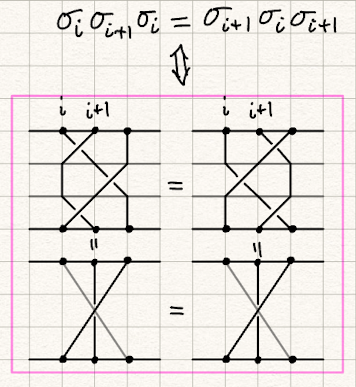
\includegraphics[width = .5\textwidth]{sketch_YB_citerion_verification.png}
    \caption{\colorbox{red}{Grayed-out strand indicates that it is behind all other strands.}}\label{fig:YB_criterion_verification}
\end{figure}

\bibliographystyle{plain}
\bibliography{references}

\end{document}